



\chapter{IIR Filter}

\section{Introduction}

\begin{figure}[h]
\centering
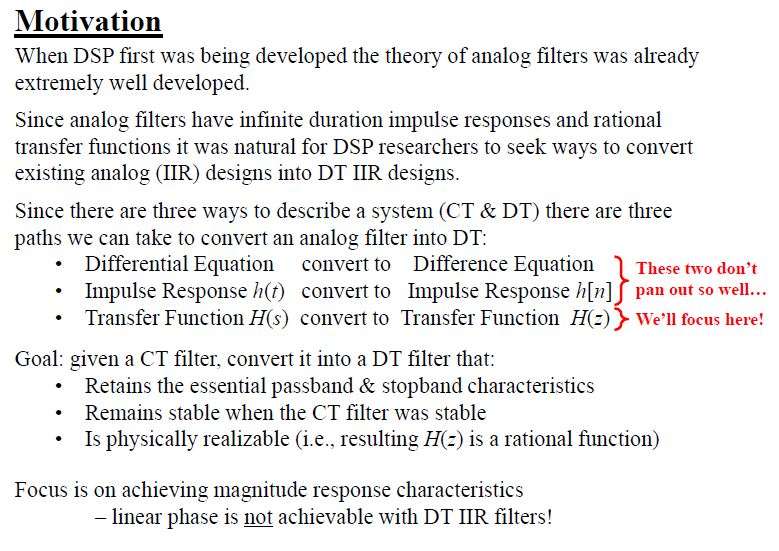
\includegraphics[width = 0.7\textwidth, frame]{Figures/IIR/Introduction}
\caption{IIR Design principle}
\label{fig:IIR:Introduction}
\end{figure}


DSP research started early in 1960 and 1970. Back then, all analog filter were implemented using analog components (resistor,inductor,capacitor,$\cdots$). What the DSP researchers hope to do is to implement these same analog filter using discrete time approach.\\


A system can be represented using 3 components: differential equation,transfer function and impulse response. What we will do is try to convert each one of them into its discrete time equivalent , and then apply the design.\\


The first 2 elements (differential equation,impulse response) don't work that much in designing IIR, so we will focus on them briefly and focus on transfer function element.

\newpage
\section{Notation}

Since we are dealing with transfer functions, and moving from analog to discrete time and frequency, we will have allot of notation illustrated in \autoref{fig:IIR:Notation_Convention}.

\begin{figure}[h]
\centering
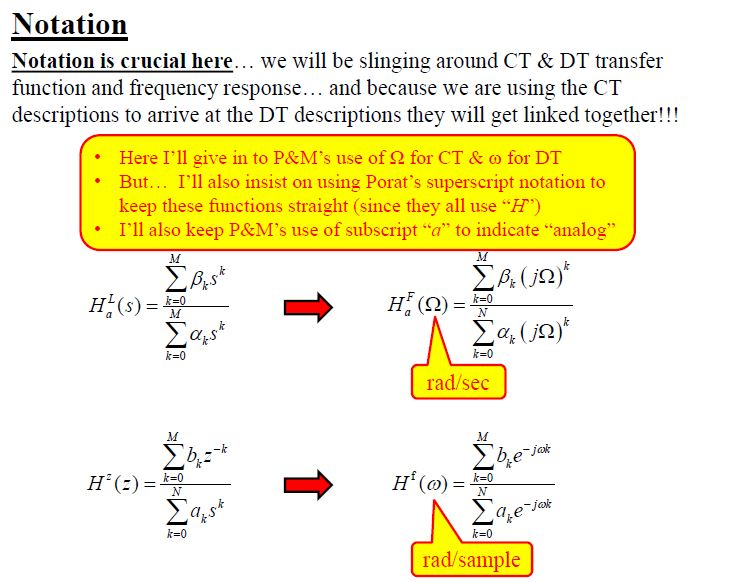
\includegraphics[width = 0.7\textwidth, frame]{Figures/IIR/Notation_Convention}
\caption{Notation Convention}
\label{fig:IIR:Notation_Convention}
\end{figure}


\newpage
\section{Difference Equation Approach}


In difference equation: we take some differential equation which represent the behaviour of some analog filter, turn it into a difference equation, then apply $z$-transforms for example to derive $H(z)$.\\

The conversion from differential equation $\rightarrow$ difference equation is done using approximation of derivative as shown in \autoref{fig:IIR:difference_eq_change_of_variables}

\begin{figure}[h]
\centering
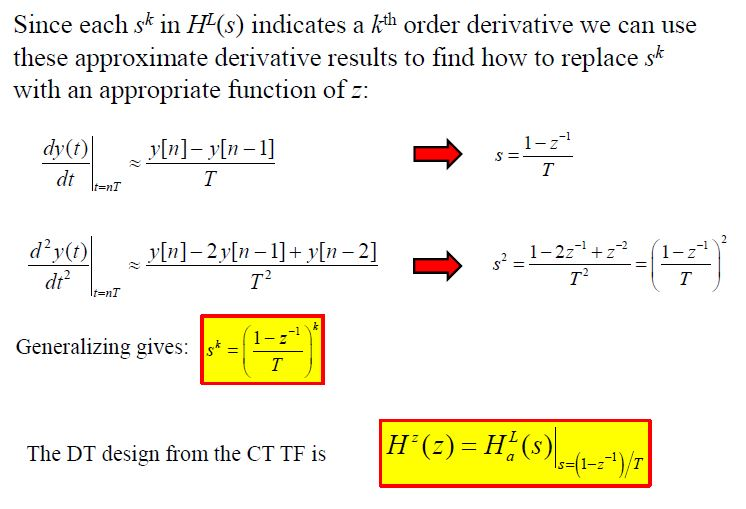
\includegraphics[width = 0.7\textwidth, frame]{Figures/IIR/difference_eq_change_of_variables}
\caption{Difference equation approach: using derivative approximation to make a change of variable from $s \rightarrow z$}
\label{fig:IIR:difference_eq_change_of_variables}
\end{figure}


Inverting the relation $s \, = \, \displaystyle\frac{1 \,  - \, z^{-1}}{T_s}$ give us $z \, = \, \displaystyle\frac{1}{1 \, - \, s \, T_s}$. Illustration using $s$-plane and $z$-plane is shown in \autoref{fig:IIR:difference_eq_change_of_variables_2}

\begin{figure}[h]
\centering
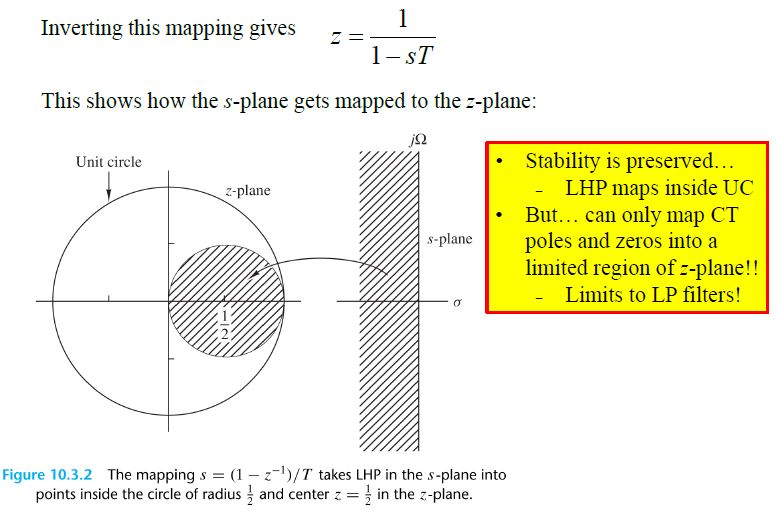
\includegraphics[width = 0.7\textwidth, frame]{Figures/IIR/difference_eq_change_of_variables_2}
\caption{Difference equation  $s \rightarrow z$ mapping using complex planes}
\label{fig:IIR:difference_eq_change_of_variables_2}
\end{figure}

Notice that in \autoref{fig:IIR:difference_eq_change_of_variables_2}, we don't have all the stable $z$-plane. So in filter design implication, we are only limited to LPF.

\section{Impulse Invariance Approach}

It takes the impulse function in the \textit{continuous frequency domain}, and turn into a \textit{discrete frequency domain} as shown in \autoref{fig:IIR:impulse_invariance}.

\begin{figure}[h]
\centering
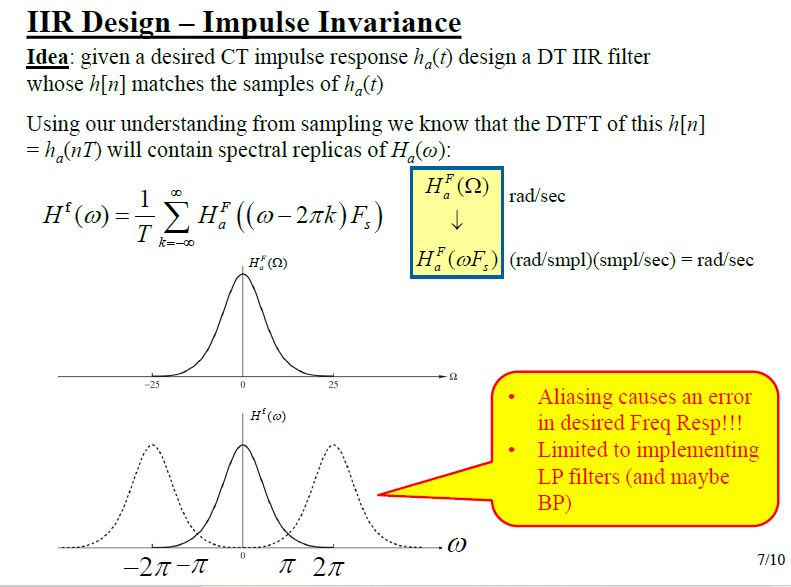
\includegraphics[width = 0.7\textwidth, frame]{Figures/IIR/impulse_invariance}
\caption{Impulse Invariance Approach: Sampling the continuous transfer function}
\label{fig:IIR:impulse_invariance}
\end{figure}

Nevertheless, in \autoref{fig:IIR:impulse_invariance} it is not very clear how to use this fact to build some discrete time system and convert it to rational transfer function. This is illustrated in \autoref{fig:IIR:impulse_invariance_2}.


\begin{figure}[h]
\centering
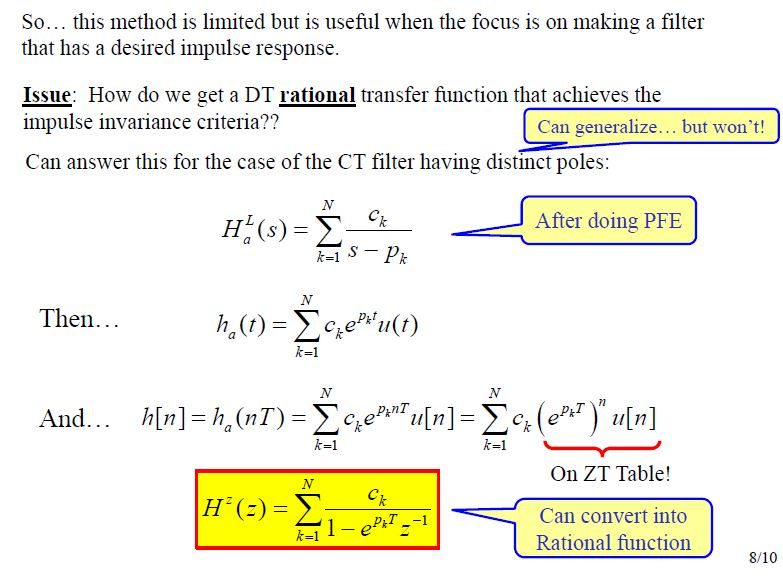
\includegraphics[width = 0.6\textwidth, frame]{Figures/IIR/impulse_invariance_2}
\caption{Impulse Invariance Approach: converting to a rational transfer function}
\label{fig:IIR:impulse_invariance_2}
\end{figure}


\newpage
\subsection{Example}

An example is shown in \autoref{fig:IIR:impulse_invariance_example}.

\begin{figure}[h]
\centering
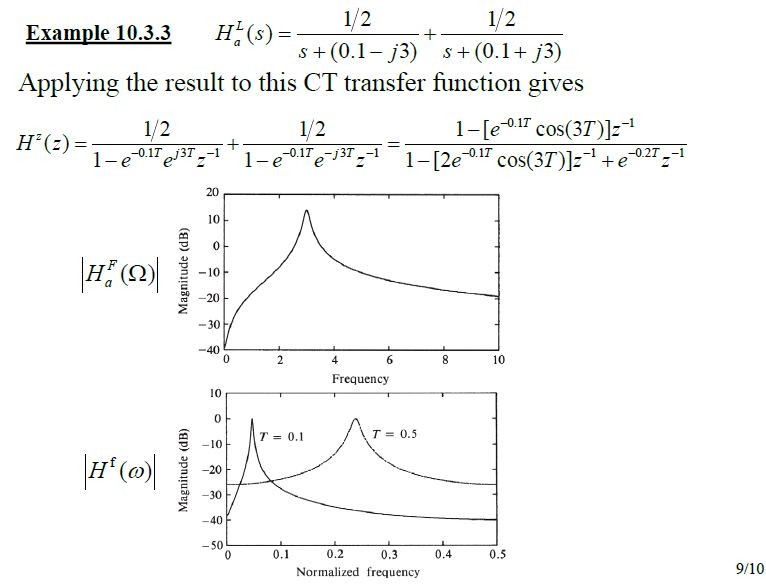
\includegraphics[width = 0.7\textwidth, frame]{Figures/IIR/impulse_invariance_example}
\caption{Impulse Invariance Approach Example}
\label{fig:IIR:impulse_invariance_example}
\end{figure}

For a bigger $T_s$, we get shift in the resonance frequency.

\newpage
\section{Bilinear Transformation}

\underline{Note:} here the term \textit{transformation} doesn't mean as in the context of Fourier or Laplace transform, but it means in the context of mapping. But this name has stuck in it in the history.\\

As a first step, what we have done before is the usage of transfer function concept. This is illustrated in \autoref{fig:IIR:bilinear_intro}.


\begin{figure}[h]
\centering
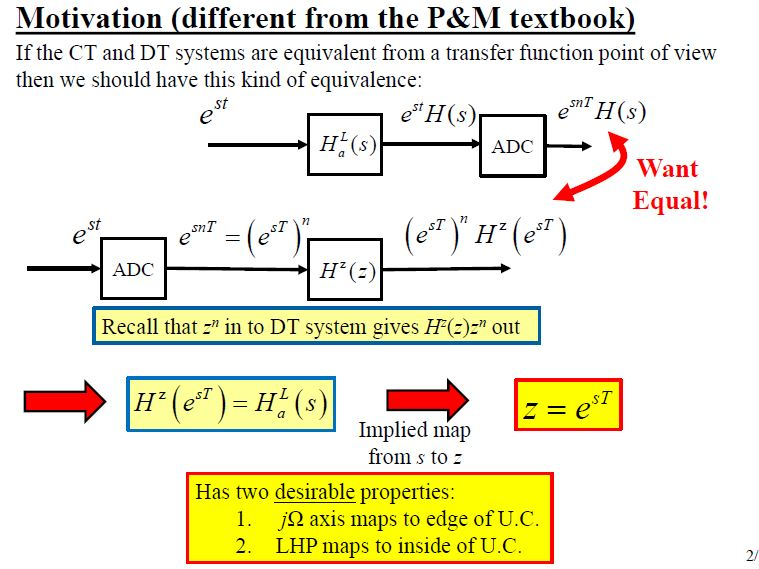
\includegraphics[width = 0.7\textwidth, frame]{Figures/IIR/bilinear_intro}
\caption{Using Transfer function concept}
\label{fig:IIR:bilinear_intro}
\end{figure}

If we want to compare, we need to use and ADC in the front end (as shown in the $\mathrm{2}^\mathrm{nd}$ row of \autoref{fig:IIR:bilinear_intro}). This lead to derive the $\mathrm{1}^\mathrm{st}$ mapping relation:

\begin{equation}
    z \, = \, e^{s\, T}
    \label{Eq:IIR:1st_mapping}
\end{equation}

\autoref{Eq:IIR:1st_mapping} have some nice properties, like stability (left half plain mapped into the uniform circle of $z-$plane). However, it causes some wrapping (which is similar to aliasing), as shown in \autoref{fig:IIR:wraping}.


\newpage
\begin{figure}[h]
\centering
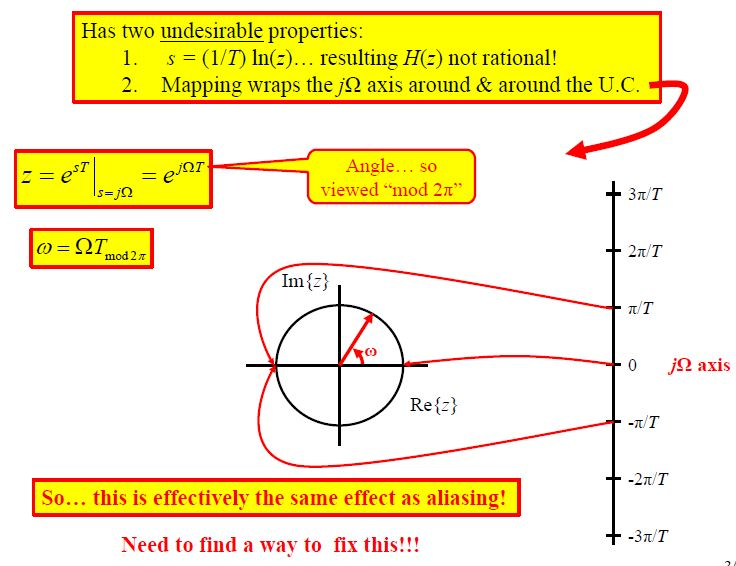
\includegraphics[width = 0.7\textwidth, frame]{Figures/IIR/wraping}
\caption{Using Transfer function concept}
\label{fig:IIR:wraping}
\end{figure}

In order to solve this problem, we need to modify the mapping. The final result will be:

\begin{equation}
    s \, = \, \left( \, \displaystyle\frac{2}{T} \, \right) \, \displaystyle\frac{z \, - \, 1}{z \, + \, 1}
    \label{Eq:IIR:2nd_mapping}
\end{equation}

\newpage
The proof of \label{Eq:IIR:2nd_mapping} is shown in \autoref{fig:IIR:proof_mapping}.

\begin{figure}[h]
\centering
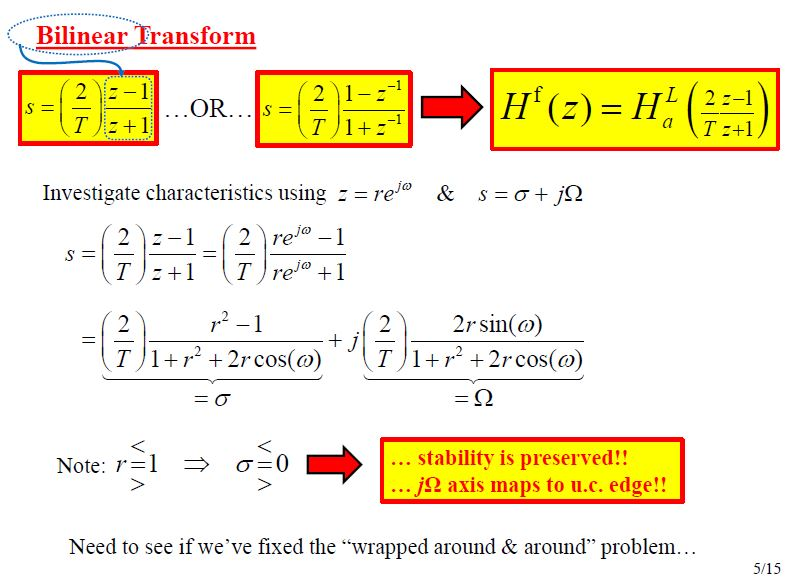
\includegraphics[width = 0.7\textwidth, frame]{Figures/IIR/proof_mapping}
\caption{Proof of Mapping}
\label{fig:IIR:proof_mapping}
\end{figure}

Concerning this proof, it isn't very clear how the researcher start with it or what is the motivation behind it, but it works.\\

Now the next step is to set $r \, = \, 1$ and $\sigma \, = \, 0$, so we can at the circle and the LHP of the $s$-plane, plugging in these values in \autoref{Eq:IIR:2nd_mapping} we get:

\begin{equation}
    \omega \, = \, 2 \, \tan^{-1} \left (\, \displaystyle\frac{\Omega \, T}{2}   \,\right)
    \label{Eq:IIR:freq_mapping}
\end{equation}

\newpage
An example of \autoref{Eq:IIR:freq_mapping} is shown in \autoref{fig:IIR:Warping_frequencies_effect}.

\begin{figure}[h]
\centering
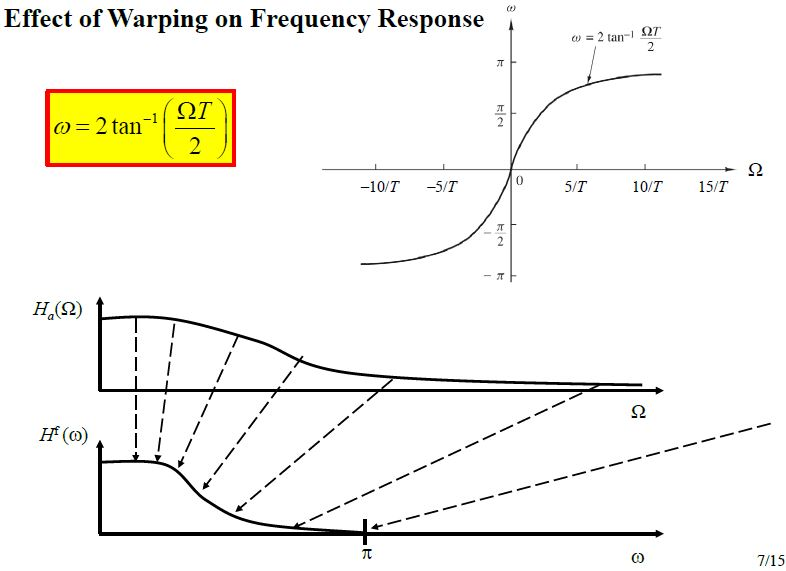
\includegraphics[width = 0.7\textwidth, frame]{Figures/IIR/Warping_frequencies_effect}
\caption{Effect Of Warping frequencies}
\label{fig:IIR:Warping_frequencies_effect}
\end{figure}

We can see that the continuous transfer function $H(\Omega)$ is spread out over all $\Omega$, and then the discrete transfer function $H(\omega)$ is squish to $\pi$, and this compression is controlled by $T_s$.

The higher the $T_s$, the more compression we get.